\documentclass[11pt]{scrartcl}
\usepackage[sexy]{evan}

\begin{document}
\title{Introduction to Functional Equations} % Beginner
\date{18 October 2016}
\maketitle

\begin{abstract}
  \sffamily\small
  So have you ever played three-player bughouse chess and been on the middle board?
  Basically, a very effective strategy is to just throw down pieces seemingly at random
  until you get something that works -- literally, just try the first thing that comes
  to mind. Other times, if this isn't working and you're running low on pieces
  {\scriptsize (and are being told to stop singing by certain people)}, then you have to
  make use of what you've got and do something fancier, but this is rare. Usually just
  slamming stuff on the board works, especially against weak opponents.

  This is all a metaphor.

  \medskip

  --- Max Schindler
\end{abstract}

\vspace{1em}
%%fakesection Notations + Acknow

Let $f\colon A \to B$ be a function.
The set $A$ is called the \vocab{domain}, and $B$ the \vocab{codomain}.
A couple definitions which will be useful:
\begin{definition}
  A function $f\colon A \to B$ is \vocab{injective} if $f(x) = f(y) \iff x=y$.
  (Sometimes also called \emph{one-to-one}.)
\end{definition}
\begin{definition}
  A function $f\colon A \to B$ is \vocab{surjective} if for all $b \in B$,
  there is some $x \in A$ such that $f(x) = b$.
  (Sometimes also called \emph{onto}.)
\end{definition}
\begin{definition}
  A function is \vocab{bijective} if it is both injective and surjective.
\end{definition}

In this handout, by ``solve over $K$''
I will mean ``find all functions $f \colon K \to K$ such
that the equation holds for all inputs in $K$''.

\subsection*{Acknowledgments}
\textsc{Thanks} to Ashwin Sah and David Stoner for detailed suggestions,
and to Ryan Kim, Kevin Qian and Franklyn Wang for comments and corrections.

\section{Synopsis}
A typical functional equation will ask you to find all functions satisfying so-and-so property, for example:
\begin{example}[USAMO 2002]
  Find all functions $f \colon \RR \to \RR$ such that $f(x^2-y^2) = xf(x) - yf(y)$ over $\RR$.
\end{example}
The answer is just $f(x) = kx$ for some constant $k$.

In any problem that asks you to ``find all $X$ satisfying $Y$'',
there are always \textbf{two} things you must do:
\begin{itemize}
  \ii check that all objects
  satisfying the condition are of the form you describe
  \ii \emph{and} prove that anything of the form
  you describe satisfies the condition.
\end{itemize}
In the context of this problem, this means you need to show that
\[ f(x^2-y^2) = xf(x) - yf(y) \quad\text{ if and only if }\quad f(x) = kx. \]
Of course the ``if'' direction is trivial in this example,
and the bulk of the work is ``only if''.
However, you should keep clear in your mind both directions,
and also remember to state that the ``if'' direction is trivial on a contest,
or you \emph{will} lose a point!
\begin{center}
  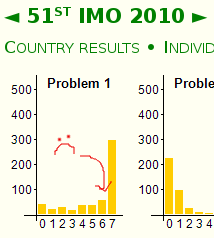
\includegraphics[scale=0.75]{6s-at-imo-edited.png}
\end{center}
In fact, I recommend structuring the opening lines of your solution as follows:
\begin{mdframed}
  \emph{Solution.} The answer is $f(x) = kx$, $k \in \RR$.
  It's easy to see that these functions satisfy
  the given equation.

  We now show these are the only solutions\dots
\end{mdframed}

\section{First Example}
For concreteness, let me start off with a standard example,
that shows a lot of the types of things that often come up in these sorts of problems.
\begin{example}[Kyrgyzstan 2012]
  \label{ex:begin}
  Find all functions $f \colon \RR \to \RR$ such that
  \[ f(f(x)^2+f(y)) = xf(x)+y \]
  for all $x,y \in \RR$.
\end{example}

\begin{soln}
  Before I begin solving the problem, can you guess what the answer is?
  Clearly, $f(x) = +x$ works.
  But there's actually a second solution: $f(x) = -x$.
  In general, a ``garden-variety'' functional equation will have $f(x) = x$ as a solution,
  but sometimes also $f(x) = 0$, $f(x) = kx$, $f(x) = x+c$, or even $f(x) = kx+c$.
  So therefore, I recommend \textbf{at the start of every problem that you start by seeing
  which if any of these functions are solutions},
  and to just keep these in your head.%
  \footnote{One reader suggests also
    checking degree $n$ polynomials in general.
    This is often easier than it seems,
    since degrees usually end up not
    matching except for finitely many $n$.}

  For this problem,
  it looks like $f(x) = \pm x$ is a solution, so we just need
  to keep in mind that we need to allow for this case.

  Now, where do we begin?
  Well, one can simply start off by plugging stuff in,
  and grabbing whatever low-hanging fruit we can.
  Usually, the first thing I try is setting all zeros; this is often helpful,
  and in general your first attempts should try to make a lot of terms vanish.
  When we do this here, we get
  \[ f(f(0)^2 + f(0)) = 0. \]
  The inner term is pretty messy, but let me for now just denote it $u$,
  i.e.\ we have some $u$ such that $f(u) = 0$.
  This is still useful, because we can use it to make things disappear!
  By plugging in $x=u$ we obtain that
  \[ f(f(y)) = y. \]
  Such an $f$ is called an \emph{involution}.
  This is good, because in fact $f$ is now automatically a bijection:
  \begin{exercise}
    Prove that if $f(f(y)) = y$, then $f$ is both injective and surjective.
    (For the ``injective'' direction, start by assuming $f(a) = f(b)$
    then do something to both sides.)
  \end{exercise}

  Of course, this is not all it gives us.
  In the given equation, we can now put $x=f(t)$
  in order to replace all the $f(x)$'s with $f(f(t))=t$'s
  (thus paradoxically we're decreasing the number of nested terms
  by adding an extra $f$ into the given!).
  This gives us:
  \begin{align*}
    f(f({\color{red} x})^2+f({\color{blue} y}))
    &= {\color{red} x}f({\color{red} x}) + {\color{blue} y} & \text{given} \\
    f(f({\color{red} f(t)})^2+f(y))
    &= ({\color{red} f(t)})f({\color{red} f(t)}) + {\color{blue} y} & \text{put $x=f(t)$} \\
    f(t^2 + f(y)) &= f(t) \cdot t + y & \text{since } f(f(t)) = t \\
    &= f(f(t)^2+f(y)) & \text{by given}.
  \end{align*}
  We arrive at the conclusion that
  \[ f(t^2+f(y)) = f(f(t)^2+f(y)). \]
  But \textbf{since $f$ is injective}
  (since it is a bijection),
  we can now conclude that
  \[ t^2 + f(y) = f(t)^2 + f(y) \implies f(t) = \pm t \]
  for every $t$!
  (This is why having injectivity is often useful.)

  There's still a little more to go, even though this looks like almost what we want.
  While we know that $f(t) = \pm t$ for every \emph{particular} $t$,
  we don't know whether the sign of $t$ can change or not:
  what if there are solutions such that $f(t) = t$ sometimes and $f(t) = -t$ other times?
  (This type of error has even received an unofficial name:
  the so-called \vocab{pointwise trap}.)

  However, this seems highly unlikely, and to that end it is not hard to dispense of.
  Suppose that $f(a) = +a$ and $f(b) = -b$ for now.
  \begin{exercise}
    Plug these into the given equation and verify that the only possibility
    is when one of them is zero.
  \end{exercise}
  Thus, we have shown that if $f$ satisfies the given, then $f(x) = \pm x$.
  And of course, the last step I warned you to not forget:
  verify that these two $f$'s are indeed solutions.
\end{soln}
\begin{remark}
  There are of course other approaches.
  Here is an outline of another one.
  After showing $f$ is an involution,
  one can simultaneously let $x = f(t)$, $y = f(u)$
  and instead obtain \[ f(t^2 + u) = t f(t) + f(u) \]
  (check this!).
  This quickly becomes a ``Cauchy equation'',
  see below and \Cref{pr:finish_up}.
\end{remark}
\begin{remark}
  Possibly helpful suggestion:
  the set of solutions you find also motivates
  which claims may be helpful to prove.
  For example, if $f(x) = x$ and $f(x) = 2-x$
  then you can't hope to prove $f(0)=0$ or $f(xy) = f(x)f(y)$,
  but it may be possible to show $f(1) = 1$ or $f$ involutive,
  for example.
\end{remark}

\section{Cauchy's Functional Equation Over $\QQ$}
For this section, all functions are $f \colon \QQ \to \QQ$.
We highly encourage the reader to try these examples on their own
before reading the solutions;
they are good practice problems!

\begin{example}[Cauchy's Functional Equation]
  Solve $f(x+y) = f(x) + f(y)$ over $\QQ$.
\end{example}
\begin{soln}
  As before we begin by examining which
  functions we think the answers are.
  Trying out the most general $f(x) = kx+c$,
  we find that $c=0$ but $k$ can be anything.
  So our guess is that the answer is $f(x) = kx$.

  We now prove this guess is right. First, all such functions clearly work.

  Now, to actually solve the problem,
  observe that we have ``one degree of freedom'':
  the family of solutions has a free variable.
  So it makes sense to set, say, $k = f(1)$
  and try to solve everything else in terms of $k$.

  We begin now by setting $x=y=0$ to derive $f(0) = 0$.
  Then, we can put $x=1$, $y=1$ to get $f(2) = f(1)+f(1) = 2k$.
  Now, $(x,y) = (2,1)$ gives $f(3) = 3k$, and so on,
  so by induction we get $f(n) = kn$ for any integer $n \ge 1$.

  What about the negative integers?
  Well, by putting $x=-y$ we get $f(x) + f(-x) = 0$, and so in fact $f$ is odd.
  Thus the result $f(n) = kn$ holds for the negative integers.

  We're still stuck with the problem of getting all of $\QQ$.
  As a thought experiment, let's see what we can do to get $f(\half)$.
  We have that
  \[ f\left(\half\right) + f\left(\half\right) = f(1) = k \]
  whence $f(\half) = \half k$.
  And now the path is clear for general $p/q$: we have
  \[ \underbrace{f(p/q) + \dots + f(p/q)}_q = f(p) = kp \]
  and hence $f(p/q) = k \cdot p/q$.
  Thus, we conclude that $f(x) = kx$ for all $x$.
\end{soln}

\begin{remark}
Notice how the choice of $\QQ$ as domain is critical:
this all works out because we are able to do induction
in order to get the function $f$ over $\ZZ$ inputs,
and then over $\QQ$.
This fails if $f \colon \RR \to \QQ$, as the next section shows.

In contrast, the choice of codomain is irrelevant,
we run into no problem if we repeat this proof for $f \colon \QQ \to \RR$.
\end{remark}


\begin{example}[Jensen's Functional Equation]
  Solve over $\QQ$: \[ f(x) + f(y) = 2f\left( \frac{x+y}{2} \right). \]
\end{example}
\begin{soln}
  This time, our preliminary checks reveal that $f(x) = kx+c$ works for any $k$ and $c$.
  (In a vague sense, the fact that $c$ is free to vary is manifested in the fact that
  plugging in all zeros yields the tautology $0=0$.)
  So now we do the following trick: we can shift the function $f$ by $c$ without changing the function.
  To be clear, this means that we rewrite the given as
  \[ \left( f(x)-f(0) \right) + \left( f(y)-f(0) \right)
  = 2\left( f\left( \frac{x+y}{2} \right) - f(0) \right). \]
  If we now let $g(x) = f(x) - f(0)$, then we derive
  \[ g(x) + g(y) = 2g\left( \frac{x+y}{2} \right) \]
  so this is the same functional equation -- but now, we know $g(0) = 0$.

  So, setting $(x,y) = (t,0)$ gives $g(t) = 2g(t/2)$.
  We might try the same trick as before with Cauchy, say setting $(x,y) = (1,2)$ to get
  \[ g(1) + g(2) = 2g(3/2) \]
  which seems non-useful until we remember we have $g(t) = 2g(t/2)$.
  Indeed, the given functional equation can be rewritten as
  \[ g(x) + g(y) = 2g\left( \frac{x+y}{2} \right) = g\left( x+y \right) \]
  with $t = x+y$.
  So $g$ satisfies Cauchy!
  \begin{exercise}
    Finish up from here.\qedhere
  \end{exercise}
\end{soln}

\begin{example}[JMO 2015/4]
  Find all functions $f\colon \QQ \to \QQ$ such that
  \[ f(x)+f(t)=f(y)+f(z) \]
  for all rational numbers $x<y<z<t$ that form an arithmetic progression.
\end{example}
\begin{soln}
  As before, we see that linear functions $f(x) = kx+c$ satisfy the condition.
  We could shift to $0$ as before if we like,
  but for this problem it will turn out to make not a difference,
  so I'll cheat and tell you to not bother.

  Now, let's clean up the equation a little by writing it as
  \begin{align*}
    f(a) + f(a+3d) &= f(a+d) + f(a+2d). \\
    \intertext{for $d > 0$. This has a lot of terms in it,
    and it'd be great if we get a lot of them to cancel each other off.
    The trick is to try to make more things cancel by writing down the shifted version}
    f(a-d) + f(a+2d) &= f(a) + f(a+d) \\
    \intertext{which follows by replacing $a$ with $a-d$. Adding:}
    f(a-d) + f(a+3d) &= 2f(a+d) \qquad \forall a \in \QQ \text{ and } d > 0.
  \end{align*}
  At this point we're actually done:
  \begin{exercise}
    Reduce this to Jensen's functional equation and complete the problem.
    (You'll need to address the case $d=0$ separately, trivial as it is.)
    \qedhere
  \end{exercise}
\end{soln}

So the main idea of this solution was that by shifting a little,
we could cause several terms to cancel off.
That leads us back to Jensen's equation.

\section{Cauchy's Functional Equation Over $\RR$}
As I alluded to earlier, the problem becomes very
different if we replace $\QQ$ by $\RR$, since
induction is no longer valid.
Actually, over $\RR$, we get new pathological (or just ``bad'')
solutions to Cauchy's equation that weren't there before.

Here's the summary of the situation:
\begin{theorem}[Cauchy + Continuous $\implies$ Linear]
  Suppose $f \colon \RR \to \RR$ satisfies $f(x+y) = f(x) + f(y)$.
  Then $f(qx) = qf(x)$ for any $q \in \QQ$.
  Moreover, $f$ is linear if any of the following are true:
  \begin{itemize}
    \ii $f$ is continuous in any interval.
    \ii $f$ is bounded (either above or below) in any nontrivial interval.
    \ii There exists $(a,b)$ and $\eps > 0$ such that $(x-a)^2 + (f(x)-b)^2 > \eps$ for every $x$
    (i.e.\ the graph of $f$ omits some disk, however small).
  \end{itemize}
\end{theorem}
It's actually pretty intuitive how to construct a bad function.
\begin{exercise}
  Construct a ``bad'' $f \colon \QQ[\sqrt2] \to \QQ[\sqrt2]$.
  Can you construct one such that $f(f(x)) = x$ as well?
\end{exercise}
I won't go into the details more than that; see my handout \emph{Monsters} for more discussion.

In general, however, if you end up with Cauchy's Functional Equation,
then very often a judicious use of the given equation will let you break free.
The relation $f(x+y) = f(x) + f(y)$ is very powerful,
and usually just using the multiplicative structure a little bit will get you what you need.
Here's an example of what I mean.

\begin{example}[Field Automorphisms of $\RR$]
  Solve over $\RR$:
  \[ f(x+y) = f(x) + f(y) \quad\text{and}\quad f(xy) = f(x)f(y). \]
\end{example}
\begin{proof}
  [Solution]
  We claim $f(x) = x$ and $f(x) = 0$ are the only solutions (which both work).
  According to the theorem, to prove $f$ is linear it suffices to show $f$ is nonnegative
  over some nontrivial interval.
  Now, \[ f(t^2) = f(t)^2 \ge 0 \] for any $t$,
  meaning $f$ is bounded below on $[0,\infty)$
  and so we conclude $f(x) = cx$ for some $c$.
  Then $cxy = (cx)(cy)$ implies $c \in \{0,1\}$, as claimed.
\end{proof}

In general, as far as olympiad contexts, the most common ways
to get from additive to linear are:
\begin{itemize}
  \ii Being able to prove bounded conditions (such as $f \ge 0$), or
  \ii The problem \emph{gives} you that the function $f$ is continuous.
  It is extremely rare that you need to prove continuity yourself;
  in fact I personally cannot think of a single functional equation in which
  continuity is a useful intermediate step.
\end{itemize}

\section{More Examples}
Here are some more examples of $\RR \to \RR$ equations.
\begin{example}
  [David Yang] \label{ex:david_yang}
  Solve over $\RR$: \[ f(x^2+y) = f(x^{27} + 2y) + f(x^4). \]
\end{example}
\begin{soln}
  For this problem, we claim the only answer is the constant function $f=0$.
  As usual our first move is to take the all-zero setting, which gives $f(0) = 0$.

  Now, let's step back: can we do anything that will make lots of terms go away?
  There's actually a very artificial choice that will do wonders.
  It is motivated by the \vocab{battle cry}:
  \begin{quote}
    \itshape ``DURR WE WANT STUFF TO CANCEL.''
  \end{quote}
  So we do the most blithely stupid thing possible.
  \emph{See that $x^2+y$ and $x^{27}+2y$ up there?}
  Let's make them equal in the rudest way possible:
  \[ x^2 + y = x^{27} + 2y \iff y = x^2 - x^{27}. \]
  Plugging in this choice of $y$,
  this gives us $f(x^4) = 0$, so $f$ is zero on all nonnegatives.

  All that remains is to get $f$ zero on all reals.
  The easiest way to do this is put $y=0$ since this won't
  hurt the already positive $x^2$ and $x^4$ terms there.
\end{soln}
This is a common trick: see if you can make a substitution that will kill off two terms.

\begin{example}[Singapore 1999]
  \label{ex:singapore}
  Solve over $\RR$:
  \[ (x-y)f(x+y) - (x+y)f(x-y) = 4xy(x^2-y^2). \]
\end{example}
\begin{soln}
  First, the $x-y$ and $x+y$ everywhere are a mess,
  so we replace them with $a = x+y$ and $b = x-y$ (this doesn't lose any information).
  Then $x^2-y^2 = ab$, and also $2x = a+b$, $2y = a-b$.
  So, the equation is just saying that
  \[ bf(a) - af(b) = ab(a^2-b^2). \]
  This looks much less terrible to work with.

  We begin our siege properly now.
  First, we might try to probe the solutions, as before.
  In this case we observe there are no linear or constant solutions.
  \begin{exercise}
    Find a nonzero function that does work.
  \end{exercise}
  We should keep this in our minds as we proceed.\footnote{%
    In general, if linear functions don't work at all
    or if one gets stuck trying to prove only linear functions work,
    it can be worth it to check degree $n$ polynomials in general.
    Again, for degree reasons there are usually only finitely many $n$ to check.}
  One other remark worth making is that the left-hand side is in fact zero
  for $f(x) \equiv cx$, which leads to an observation that
  if $f$ is a solution, then so is $f+2016x$, say.
  This tells us a bit more about what the solution space might look like.

  Plugging in $a=b=0$, then we get $0=0$, not helpful.
  Plugging in just one zero term $a=0$ is more fruitful: we derive
  $bf(0) = 0$, so $f(0) = 0$.

  Next, assume $a,b \neq 0$.
  We do the following nice trick:
  if we divide by $ab$, we obtain
  \[ \frac{f(a)}{a} - \frac{f(b)}{b} = a^2 - b^2. \]
  You'll notice that the $a$ and $b$ terms are completely isolated now!
  That is, we can write
  \[ \frac{f(a)}{a} - a^2 = \frac{f(b)}{b} - b^2. \]
  This is enough to imply that $\frac{f(a)}{a} - a^2 = c$ for some constant $c$,
  whenever $a \neq 0$; hence $f(x) = x^3 + cx$ for some $c$.
  Initially we only know this for $x \neq 0$,
  but it holds for $x=0$ as well since $f(0) = 0$.

  And now, we observe that these solutions all work, and we're done.
\end{soln}

\section{Three More Tricks}
Here are three more tricks that are frequently useful.

\begin{itemize}
  \ii \vocab{Tripling an involution}.
  If you know something about $f(f(x))$,
  try applying it $f(f(f(x)))$ in different ways.
  For example, if we know that $f(f(x)) = x+2$,
  then we obtain $f^3(x) = f(x+2) = f(x)+2$.

  \ii \vocab{Isolated parts}.
  When trying to obtain injective or surjective,
  watch for ``isolated'' variables or parts of the equation.
  For example, suppose you have a condition like
  \[ f(x+2xf(y)^2) = yf(x) + f(f(y)+1) \]
  (I made that up).
  Noting that $f \equiv 0$ works, assume $f$ is not zero everywhere.
  Then by taking $x_0$ with $f(x_0) \neq 0$,
  one obtains $f$ is injective.
  (Try putting in $y_1$ and $y_2$.)

  Proving surjectivity can often be done in similar spirit.
  For example, suppose
  \[ f(f(y)+xf(x)) = y+f(x)^2. \]
  By varying $y$ with $x$ fixed we get that $f$ is surjective,
  and thus we can pick $x_0$ so that $f(x_0) = 0$
  and go from there.
  Surjectivity can be especially nice if every $y$
  is wrapped in an $f$, say; then each $f(y)$ just becomes
  replace by an arbitrary real.

  \ii \vocab{Exploiting ``bumps'' in symmetry}.
  If some parts of an equation are symmetric and others are not,
  swapping $x$ and $y$ can often be helpful.
  For example, suppose you have a condition like
  \[ f(x+f(y)) + f(xy) = f(x+1)f(y+1) - 1 \]
  (again I made that up).
  This equation is ``almost symmetric'',
  except for a ``bump'' on the far left where $f(x+f(y))$ is asymmetric.
  So if we take the equation with $x$ and $y$ flipped
  and then eliminate the common terms,
  we manage to obtain \[ f(x+f(y)) = f(y+f(x)). \]
  If we've shown $f$ is injective, we are even done!
  So often these ``bumps'' are what let you solve a problem.
  (In particular, don't get rid of the bumps!)
\end{itemize}


\section{Heuristics}
At the beginning of a problem:
\begin{itemize}
  \ii Figure out what the answer is.
  For many problems, plug in $f(x) = kx+c$ and find which $k$, $c$ work.
  It may also be worth trying general polynomial functions.
  \ii Make obvious optimizations (like scaling or shifting).
  \ii Plug in $x=y=0$, $x=0$ into the givens, et cetera.
  See what the most simple substitutions give first.
\end{itemize}
Once you've done these obvious steps, some other things to try:
\begin{itemize}
  \ii The \textbf{battle cry} ``DURR WE WANT STUFF TO CANCEL''.
  Plug in things that make lots of terms cancel (as in \Cref{ex:david_yang})
  or that make lots of terms vanish (think $x=y=0$).
  \ii Watch for opportunities to prove injectivity or surjectivity,
  for example using \textbf{isolated parts}.
  \ii Watch for \textbf{bumps in symmetry} and \textbf{involutions}.
  \ii For equations over $\NN$, $\ZZ$, or $\QQ$, induction is often helpful.
  It can also be helpful over $\RR$ as well.
  The triggers for induction are the same as any other olympiad problem:
  you can pin down new values to previous ones.
  \ii It may help to rewrite the function in terms of other functions,
  like we did in \Cref{ex:singapore}, where looking at $g(x) = f(x) / x$ was useful.
  Actually, the ``shift to zero'' trick is a special case of this as well.
\end{itemize}
Some other small tricks I should mention:

Endgame techniques:
\begin{itemize}
  \ii Often, you'll get something like $f(x)^2 = x^2$
  or $f(x) \in \{0,x\}$ or something of this sort;
  see the \textbf{pointwise trap} at the end of \Cref{ex:begin}.
  When this happens, make sure you do not automatically assume $f(x) = x$ for each $x$;
  this type of equality holds only for each individual $x$.
  \ii \textbf{Check the solutions work!}
  Don't get a $6$ unnecessarily after solving the problem
  just because you forget this trivial step.
\end{itemize}

This is one useful viewpoint for solving equations.
There is a second spiritual perspective of trying to construct ``pathological'' functions
that satisfy the problem conditions, much like when we constructed the counterexample
to Cauchy's functional equation in $\QQ[\sqrt2] \to \QQ[\sqrt2]$.
This is covered in my more advanced \emph{Monsters} handout.

\eject

\section{Practice Problems}
\begin{problem}
  [Taiwan IMO Training]
  Find all continuous functions $f \colon \RR \to \RR$
  such that  for any real $x$ and $y$,
  \[ f(f(x+y)) = f(x) + f(y). \]
\end{problem}

\begin{problem}
  [Iran TST 1996]
  Find, all functions $f\colon \RR \to \RR$ satisfying
  \[ f(x^2+y) = f(f(x)-y) + 4f(x)y \]
  for all real numbers $x$ and $y$.
\end{problem}

\begin{problem}
  Solve $f(t^2+u) = tf(t) + f(u)$ over $\RR$.
  \label{pr:finish_up}
\end{problem}

\begin{problem}
  Solve $f(m+n)=f(m)+f(n)+mn$ for $f \colon \NN \to \NN$.
  % Canada handout
\end{problem}

\begin{problem}
  [Taiwan TST Quiz 2014]
  Find all (strictly) increasing functions $f$ from the nonnegative integers
  to the integers satisfying $f(2)=7$ and \[ f(mn) = f(m) + f(n) + f(m)f(n) \]
  for all nonnegative integers $m$ and $n$.
\end{problem}

\begin{problem}
  [IMO 2010/1]
  Solve $f(\left\lfloor x\right\rfloor y)=f(x)\left\lfloor f(y)\right\rfloor$ over $\RR$.
\end{problem}

\begin{problem}
  [USAMO 2002/4]
  Solve over $\RR$: \[ f(x^2-y^2) = xf(x) - yf(y). \]
\end{problem}

\begin{problem}
  [ELMO 2014]
  Find all triples $(f,g,h)$ of injective functions from the set of real numbers to itself satisfying
  \begin{align*}
    f(x+f(y)) &= g(x) + h(y) \\
    g(x+g(y)) &= h(x) + f(y) \\
    h(x+h(y)) &= f(x) + g(y)
  \end{align*}
  for all real numbers $x$ and $y$.
\end{problem}

\begin{problem}
  [ELMO Shortlist 2013 A3]
  Find all $f\colon \RR \to \RR$ such that for all $x,y\in \RR$,
  \[ f(x)+f(y) = f(x+y) \quad\text{and}\quad f(x^{2013}) = f(x)^{2013}. \]
\end{problem}

\begin{problem}
  [IMO 2012/4]
  Find all functions $f\colon \ZZ \to \ZZ$ such that,
  for all integers $a,b,c$ that satisfy $a+b+c=0$, the following equality holds:
  \[f(a)^2+f(b)^2+f(c)^2=2f(a)f(b)+2f(b)f(c)+2f(c)f(a).\]
\end{problem}

\begin{problem}
  [USAMO 2016/4]
  Find all functions $f\colon \RR \to \RR$
  such that for all real numbers $x$ and $y$,
  \[ (f(x)+xy)\cdot f(x-3y)+(f(y)+xy)\cdot f(3x-y)=(f(x+y))^2. \]
\end{problem}

\end{document}
